\lvli{Introduction}

In this experiment we analyzed the behavior of an FBG (Fiber Bragg Grating). The FBG uses the Bragg Mirror, which is a specific type of photonic crystal that acts as a mirror for a given range of frequencies. This photonic crystall can be modeled as a multilayer film where two materials with different refractive index are alternated. Imagining an ideal Bragg mirror the reflected wavelength is defined as $\lambda_{BRAGG} = \frac{2\pi}{k_{BRAGG}}$ where $k_{BRAGG}$ it is the propagation constant of the phase and respects this rule $k_{BRAGG} \cdot (L_1 + L_2) = m \cdot \pi$ with $m \in \mathbb{N}$ and $L_1, L_2$ are the two lengths of the films. By inserting a Bragg mirror into the fiber we obtain a mechanical coupling between the two in particular in compression and elongation, in fact pulling the fiber is also pulled the mirror and then modified the period $(L_1 + L_2)$ which that turns into a changes of $\lambda_{BRAGG}$. From this physical effect we can then relate elongation with the reflected frequency. This mirror, however, is also sensitive to temperature variations, in fact, in addition to creating an expansion or compression of the period, it introduces a variation of the silica refraction index induced by the thermo-optic effect.

The setup we use is composed of an optical amplifier that produces broadband light that is inserted into a fiber containing an FBG, the light that is reflected then passes through an optical circulator that sends it to a spectrum analyzer (Fig.\ref{fig:setup}).
\begin{figure}[h]
    \centering
    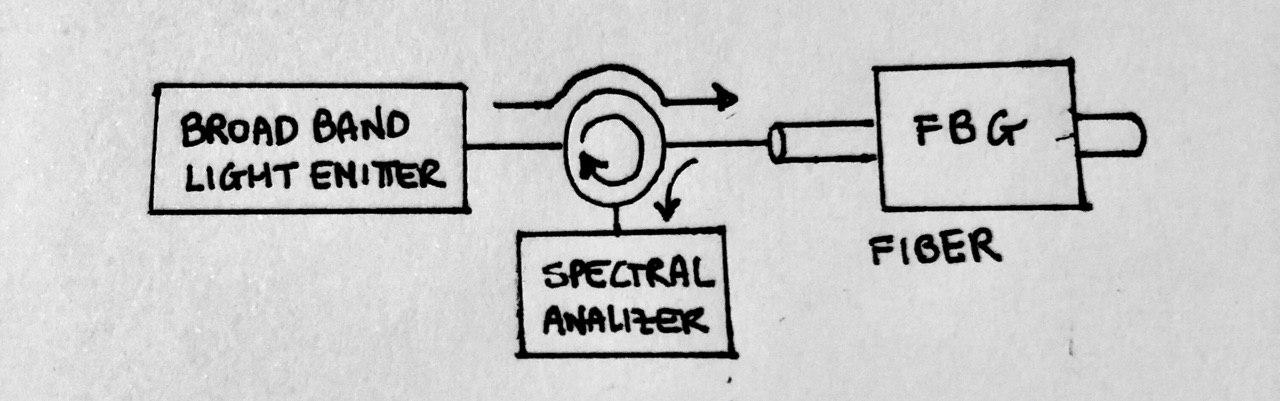
\includegraphics[scale=0.3]{img/setup.jpg}
    \caption{Setup.}
    \label{fig:setup}
\end{figure}

What is done in this experiment is to measure the reflected wave frequency according to the applied elongation. In this case the elongation is performed by turning a circular manual tensor (ring): each rotation corresponds to an elongation of $0.5 [mm]$ and on the ring there are 50 notches and therefore we have an elongation of $0.01 [mm]$ for notch. Our fiber started from a length of $14 [mm]$ and we elongated it by $0.75 [mm]$. The measurements we have performed are shown in (Tab.\ref{table:measures}), where for each rotation the value of the reflected frequency calculated by eye was reported. The table has three measuring columns because more consecutive measurements have been made starting from $14 [mm]$ and reaching $14.75 [mm]$ then going back to $14 [mm]$ and then returning to $14.75 [mm]$. The table also specifies with $(x)$ the measurements where the spectrum was stored for computer analysis.
\begin{table}[h]
  \centering
  \begin{tabular}{c|c|c|c}
      Position [mm]  &  $\lambda_B$  [nm]  &  $\lambda_B$  [nm]  &  $\lambda_B$  [nm]  \\
      \hline
      14     &  1534,691     &  1534,682(x)  &  1534,682     \\
      14.05  &  1534.861     &  1534.87      &  1534.861     \\
      14.1   &  1535.032     &  1535.032     &  1535.041(x)  \\
      14.15  &  1535.229     &  1535.186     &  1535.212     \\
      14.2   &  1535.391     &  1535.357     &  1535.391(x)  \\
      14.25  &  1535.604(x)  &  1535.562(x)  &  1535.587     \\
      14.3   &  1535.784     &  1535.749     &  1535.767(x)  \\
      14.35  &  1535.937     &  1535.92      &  1535.946     \\
      14.4   &  1536.125     &  1536.108     &  1536.108(x)  \\
      14.45  &  1536.305     &  1536.262     &  1536.305     \\
      14.5   &  1536.509(x)  &  1536.45 (x)  &  1536.467(x)  \\
      14.55  &  1536.663     &  1536.646     &  1536.646     \\
      14.6   &  1536.851     &  1536.851     &  1536.842(x)  \\
      14.65  &  1537.03      &  1537.005     &  1537.005     \\
      14.7   &  1537.184     &  1537.184     &  1537.184(x)  \\
      14.75  &  1537.389(x)  &  1537.389     &  1537.38      \\

  \end{tabular}
  \caption{Measures.}
  \label{table:measures}
\end{table}
From a first analysis we obtain the curve shown in (Fig.\ref{fig:firstAnalisy}).
\begin{figure}[h]
    \centering
    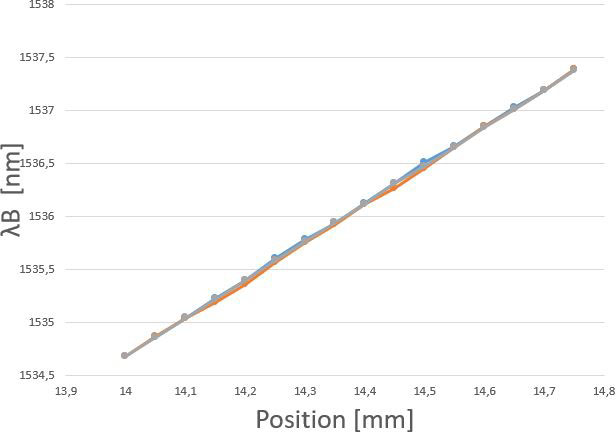
\includegraphics[scale=0.7]{img/firstAnalisy.jpg}
    \caption{First analisy.}
    \label{fig:firstAnalisy}
\end{figure}


\newpage
\lvli{Analysis}
First of all, the 13 files were imported. They contain the data related to the spectral measured by the spectrometer and contain: the two values of starting frequency and frequency step in THz; and then the list of reflected power values read in dB. The importation was made by converting the frequency values into wavelength values through the physical relation $\lambda = \frac{c_0}{f}$, to each of these values the corresponding power value has been assigned as shown in (Fig.\ref{fig:spectralPower}). From this figure it is also possible to clearly identify the peak to be analyzed, since while the signal has values lower than $-50[dB]$ and it has a value of approximately $-30[dB]$.
\begin{figure}[h]
    \centering
    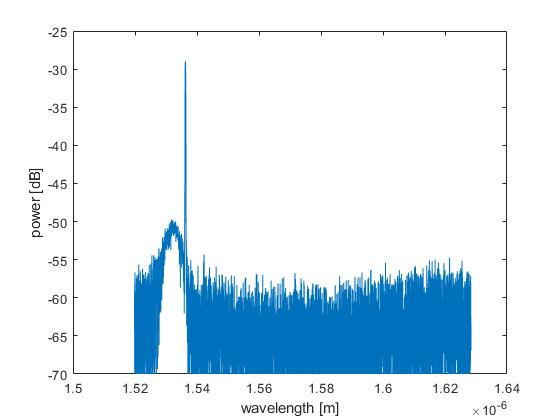
\includegraphics[scale=0.7]{img/spectralPower.jpg}
    \caption{Spectral power for 14[mm] of elongation.}
    \label{fig:spectralPower}
\end{figure}

At this point, for each file, the value of the wavelength corresponding to the maximum point is searched; to improve the analysis an interpolation of the points is performed through a quadratic function. A key point was to choose which points to consider in the approximation.
The selection of the points was made by choosing all the points that are above 90\% of the peak as we can see from the figure (Fig.\ref{fig:peak}) checking to have at least 4 points of analysis that correspond to one point more than degrees of freedom (3).
\begin{figure}[h]
    \centering
    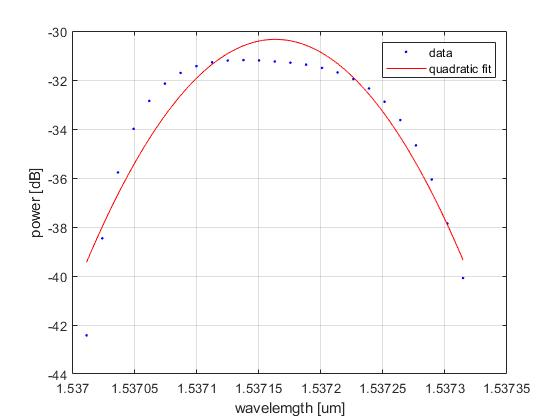
\includegraphics[scale=0.7]{img/peak.jpg}
    \caption{Quadratic approximation for the points above the 90\% of maximum value of the function.}
    \label{fig:peak}
\end{figure}

We then calculated the elongation values by setting our value of $14 [mm]$ as 0, thus obtaining a maximum elongation value of $0.75 [mm]$. At this point we calculated the strain by dividing these values by the rest length of the fiber $L = 310.5 [mm]$ which we subsequently correlated with the previously measured peaks as shown in the graph (Fig.\ref{fig:spins}).
\begin{figure}[h]
    \centering
    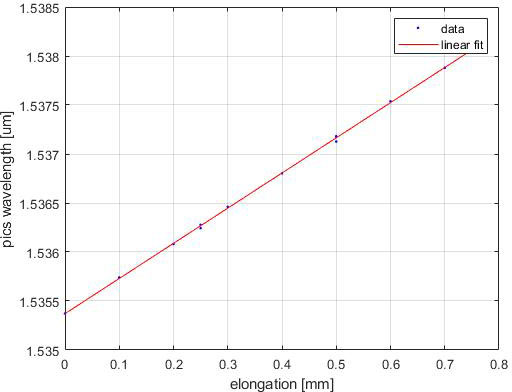
\includegraphics[scale=0.7]{img/spins.jpg}
    \caption{Elongation.}
    \label{fig:spins}
\end{figure}
From here we can obtain the angular coefficient that takes the unit of measure of:
$$\frac{\lambda}{strain}\left[\frac{\mu m}{\epsilon}\right] = \frac{\lambda}{strain}\left[\frac{pm}{\mu\epsilon}\right]$$
and it is
$$a = \frac{\Delta \lambda}{ \Delta strain} = 1.114 \left[\frac{pm}{\mu\epsilon}\right]$$
which corresponds to our value of sensitivity:
$$s = a = 1.1 \left[\frac{pm}{\mu\epsilon}\right]$$

To estimate the uncertainty provided by the sensor we can exploit the deviation that the points have in the y-axis from the function with which we have made the fit $rmse = 1.68\cdot10^{-5} [\mu m]$. Applying the correction where $M = 2$ are the points of freedom and $N = 13$ are the points taken $q = \frac{rmse}{\sqrt{N - M}} [\mu m]$ and inverting the relationship with the angular coefficient we obtain:
$$e = \frac{q \cdot 10^{6} [pm]}{a \left[\frac{pm}{\mu\epsilon}\right]} = 5 [\mu\epsilon]$$

\newpage
\lvli{Conclusion}
The performance of the data collected was excellent because they produced a linear trend as we expected with a deviation of $rmse = 1.6 \cdot 10^{-5}[\mu m]$.

The uncertainty $e = 5 [\mu\epsilon]$ is slightly higher than the typical value of $1 [\mu\epsilon]$ compared to the usual sensors, but we can not make more precise evaluations because we do not have the specific data of that sensor.

The value obtained is very similar to the typical values for sensors of this type:
$$s =  1.1 \left[\frac{pm}{\mu\epsilon}\right] \approx 1.2 \left[\frac{pm}{\mu\epsilon}\right]$$
this difference in value can be given by the uncertainty of the measurements made on the length of the fiber and on the rotations made by the tensor, in addition there is also a component that depends on temperature, even if of minor influence, since the experiment it lasted about two hours and then the room had the chance to warm up.
